
\documentclass[10pt]{report}


\usepackage[pdftex]{graphicx}
\usepackage{url} 
\usepackage[dvips, bookmarks, colorlinks=false, pdfborder={0 0 0}, pdftitle={<pdf title here>}, pdfauthor={<author's name here>}, pdfsubject={<subject here>}, pdfkeywords={<keywords here>}]{hyperref} 
\usepackage[final]{pdfpages}
\usepackage{multirow}
\usepackage[table]{xcolor} 
\usepackage{subfigure}
\usepackage{booktabs}


\newtheorem{example}{Example}[section]
\newtheorem{defn}{Def}
\newcommand{\ESIM}{\textsc{E}\small{\texttt{SIM}}~}
\newcommand\T{\rule{0pt}{3.1ex}}		% To add space b/w words and top \hline
\renewcommand{\figurename}{Fig.}

\newcommand\counter[1]{\arabic{#1} \stepcounter{#1}}
\newcounter{syscall}
\title{XOS \\ eXperimental Operating System \\
Version 1.0}
\author{Dr. K. Muralikrishnan  \\ \texttt{kmurali@nitc.ac.in} \\ {NIT Calicut} }


\begin{document}

\maketitle
\pagebreak

%......................Table of Contents............................%
\thispagestyle{plain}

\tableofcontents
\pagebreak

\chapter{Introduction}
\label{chp:osintro}

XOS (Experimental Operating System) is an experimental operating system  which is designed to be run on the  XSM  (Experimental String Machine) architecture which is a simulated machine hardware. XOS is intended as an instructional tool to help students learn essential concepts of an operating system. 
\vspace{0.1in} \\
XOS is programmed using a custom language, SPL (System Programmer's Language) which compiles to XSM compatible code. (Refer ... ) Application programs for XSM are written in APL (Application Programmer's Language). (Refer ... ) 
\vspace{0.1in} \\
The programs, data and operating system code is stored on a disk which has an XFS (Experimental File System) in it. (Refer ...)\\

The various functionalities of XOS include
\begin{itemize}
\item \textbf{Process Management}, includes scheduling and dispatching processes to the CPU. XOS is capable of \textit{multiprogramming} (the ability to run more than one process.  simultaneously). Refer ...
\item \textbf{Memory Management}, involves allocating memory for processes, demand paging (loading memory pages from the disk as and when required). Refer ...
\item \textbf{System Calls}. XOS provides various system calls for the user processes to execute certain kernel level operations. Refer ...
\end{itemize} 


\chapter{Memory Organization}
\label{chp:memoryorg}
\index{Memory Organization}

The operating system organizes memory as given below:
\begin{figure}[htp!] \small
	\centering
	\begin{tabular}{|c|c|c|c|}
	\toprule
		\textbf{Page No.} & \textbf{Contents} & \textbf{Word Address} & \textbf{$\#$ of words}\\
	\toprule
		0   & \hyperref[lbl:romcode]{ROM Code} 		& 0 -- 511 & 512\\ \hline 
		1   & \hyperref[lbl:oscode]{OS Startup code} 	& 512 -- 1023 & 512 \\ \hline 
		\multirow{5}{*}{2} 
			& \hyperref[lbl:pgtbl]{Per-Process Page Tables}   & 1024 -- 1279 & 256\\ \cline{2-4} 
			& \hyperref[lbl:memlst]{Memory Free List}  & 1280 -- 1343 & 64  \\ \cline{2-4}
			& \hyperref[lbl:gft]{System-wide Open File Table}  & 1344 -- 1471 & 128 \\ \cline{2-4} 
			& Unallocated & 1472 -- 1535 & 64\\ \hline 
		3 & \multirow{2}{*}
			{\hyperref[lbl:disklst]{Ready List of PCBs}} & \multirow{2}{*}{1536 -- 2559} & \multirow{2}{*}
			{1024}\\ \cline{1-1} 
		4 & 				&  & \\ \hline 
		5 & \hyperref[lbl:fat]{File Allocation Table} & 2560 -- 3071 &  512 \\ 
		\hline
		6 & \hyperref[lbl:fat]{Disk Free List} & 3072 -- 3583 &  512 \\ 
		\hline
		7 & \hyperref[lbl:fat]{Page Fault Handler} & 3584 -- 4095 &  512 \\ 
		\hline
		8 & \hyperref[lbl:fat]{Timer Interrupt Routine} & 4096 -- 4607 &  512 \\ 
		\hline
		9 & \hyperref[lbl:fat]{Interrupt 1 Routine} & 4608 -- 5119 &  512 \\ 
		\hline
		10 & \hyperref[lbl:fat]{Interrupt 2 Routine} & 5120 -- 5631 &  512 \\ 
		\hline
		11 & \hyperref[lbl:fat]{Interrupt 3 Routine} & 5632 -- 6143 &  512 \\ 
		\hline
		12 & \hyperref[lbl:fat]{Interrupt 4 Routine} & 6144 -- 6655 &  512 \\ 
		\hline
		13 & \hyperref[lbl:fat]{Interrupt 5 Routine} & 6656 -- 7167 &  512 \\ 
		\hline
		14 & \hyperref[lbl:fat]{Interrupt 6 Routine} & 7168 -- 7679 &  512 \\ 
		\hline
		15 & \hyperref[lbl:fat]{Interrupt 7 Routine} & 7680 -- 8191 &  512 \\ 
		\hline
		16 &  &  &  512 $\times$ 48\\ 
		\vdots & INIT and User Programs & 8192 -- 32767 &    = 24576 \\
		63 &  &  & \\  
		\hline
	\end{tabular}
	\caption{Outline of the main memory}
	\index{Memory!Organization}
\end{figure}
\begin{itemize}
	\item \textbf{ROM Code}, Read Only Memory is hard coded assembly code which loads the opearting system startup code from the disk. Refer  ... 
	\item \textbf{OS Startup code}, loads the INIT process to memory, data structures like FAT and Disk Free List, and Interrupt Routines from the disk. Refer ...
	\item \textbf{Per-Process Page Tables}, used for address translation of logical addresses to physical address. Refer ...
	\item \textbf{Memory Free List}, is a list of free memory locations in the memory. Refer ...
	\item \textbf{System-wide Open File Table}, contains a details of files which are opened by the processes. Refer ...
	\item \textbf{Ready List of PCBs}, is a list of Process Control Blocks (Refer ...), which indicates the ready and terminated processes. Refer ...
	\item \textbf{File Allocation Table}, contains details about files stored on the disk, Refer ...
	\item \textbf{Disk Free List}, contains details about used and used blocks in the disk, Refer ...
	\item \textbf{Page Fault Handler}, contains the kernel code to be executed during a page fault exception
	\item \textbf{Timer Interrupt Routine}, contains the kernel code to be executed during a timer interrupt. Refer ... 
	
	\item \textbf{Interrupt Routines}, contains kernel code to be executed during interrupts (1 to 7). Refer ...
	\item \textbf{INIT and User Programs}, is the memory space allocated for user programs in execution.
\end{itemize}

\chapter{OS Startup}
\label{chp:osstartup}



\section{ROM Code}
\label{lbl:romcode}
It is a hard coded assembly level code present in page 0 of the memory. It is known as the ROM (Read Only Memory) code because in an actual machine it is burnt in the hardware. When the machine boots up, this code is executed. This code has the basic functionality of loading block 0 of the disk (containing the OS startup code) into page 1 of the memory and to set the \texttt{IP} register value to 512 and start execution.


\section{\texttt{INIT} Process}
\index{\texttt{INIT} Process}
\label{lbl:INITprocess}
The Operating System starts execution with only a single user program - the \texttt{INIT} process. The \texttt{INIT} process code resides in the disk blocks 13 -- 15 . During execution of the \texttt{INIT} process, 3 pages will be used for the code, and the 4th page of the logical address space will be used as the stack. The OS Startup Code is responsible for loading the \texttt{INIT} process into memory and starting its execution.


\section{OS Startup Code}
\index{OS Startup Code}
\label{lbl:oscode}
When the machine boots up, the \textit{ROM} code loads the \textit{OS startup code} into the  memory. The OS startup code (instructions in page 1 of the memory) starts execution in the \textit{Kernel mode}. It performs the following functions.
\begin{itemize}
	\item It loads the Page Fault Exception Handler and Interrupt Service Routines from the blocks 1--9 of the disk into pages 7--15 of the memory.
	\item It loads the FAT from the block 10 of the disk into page 5 of the memory.
	\item It loads the Disk Free List from the block 11 of the disk into page 6 of the memory.
	\item It generates the Memory Free List and stores it in words 256--319 of page 2 of the memory.
	\item It loads the \texttt{INIT} process code from the hard disk into the memory by performing the following steps:
	\begin{itemize}
		\item Sets the page table of the \texttt{INIT} process with disk address pointing to the code of the \texttt{INIT} process. (Refer ...)		
		\item Update the ready list and \texttt{PID} register.
		\item Set the required page table entries.
		\item Set the values of SP, BP and \texttt{IP} with values 1536 , 1536 and 0 respectively.
	\end{itemize}
	\item Switch from \textit{Kernel mode} to \textit{User mode}.\footnote{This can be achieved by  \texttt{IRET} instruction.}
\end{itemize}

\textbf{Note}: All addresses are absolute addresses in Kernel mode. 

Once the OS Startup is completed, the page in which the OS Startup Code resides in memory (Page 1) is used for loading files from the disk.


\chapter{Process Management}
\label{chp:process}
\index{Process}

\section{Introduction}
Any program in its execution is called a \textbf{process}. Processes will be loaded into memory before they start their execution. Each process occupies \textbf{atmost 4 pages} of the memory. The processor generates logical addresses with respect to a process during execution, which is translated to the physical address. This translation is done by the machine using page tables, Refer ... \\ 

The XSM architecture supports demand paging and so the machine does not fix the number of processes that can be run on it. However XOS has limited the number of process running simultaneously to 32, due to limitiations in number of PCBs in the Ready List (Refer ...) and the number of Per-Process Page Tables (Refer ...)\\




\section{Process Structure}
\index{Process!Structure}
A process in the memory has the following structure.
\begin{itemize}
	\item \textbf{Code Area :} \index{Process!Code Area} These are pages of the memory that contain the executable code loaded from the disk. 
	\item \textbf{Stack :} This is the user stack used for program execution. The variables and data used during execution of program is stored in the stack. It grows in the direction of increasing word address.
\end{itemize}

Figure~\ref{fig:process structure} shows the process structure. \\

\begin{figure}[htp!] 
	\centering
	\begin{tabular}{|c|} 
		\textbf{Contents}    \\ \cline{1-1}
		\multirow{2}{*}{Code} \\
				       \\ \cline{1-1}
		\noalign{\smash{\llap{\lower2pt\hbox{\tt BP$\longrightarrow$}}}}
		 \\
	  \\
		\noalign{\smash{\llap{\raise2pt\hbox{\tt $\bigg \downarrow$ }}}}
		Stack  \\ \cline{1-1}
		\noalign{\smash{\llap{\lower2pt\hbox{\tt SP$\longrightarrow$}}}}
	\end{tabular}
	\caption{Logical Address Space of a Process}
	\label{fig:process structure}
\end{figure}




\section{Process Control Block (PCB)}
\label{sec:pcb}
\index{Process Data Structures!Process Control Block}
It contains data pertaining to the current state of the process. The size of the PCB is \textbf{32 words}. Refer figure~\ref{fig:PCB}.\\


	\begin{figure}[htp!]
		\centering
		\begin{tabular}{|c|c|c|c|c|c|c|c|c|c|}
			\hline
			0 & 1 & 2 & 3 & 4 & 5 & 6 & 7 -- 14 & 15 - 30 &  31 \\
			\hline
			PID & STATE & BP & SP & IP & PTBR & PTLR & R0 -- R7 & Per-Process & Free\\ & & & & & & & & Open File Table &   \\
			\hline
		\end{tabular}
		\caption{Structure of Process Control Block}
		
	\end{figure}

 \subsection{Process Identifier (PID)}
 The process identifier is a number from 0 to 31, which identifies the processes in memory. The PID of the current process can be calculated from the \texttt{PTBR} register.
 
	 \subsection{Process State} 
	 The process state corresponding to a process, indicated by \texttt{STATE} in the PCB stores the state of that process in the memory. A process can be in one of the following states. 
	\begin{itemize}
		\item \textbf{0} for \textit{terminated}, i.e. process has completed execution
		\item \textbf{1} for \textit{ready}, i.e. process is waiting for the CPU to start execution.
		\item \textbf{2} for \textit{running}, i.e. the process is currently running in the CPU
	\end{itemize}
	
	  \subsection{Registers} 
\begin{itemize}
	\item \textbf{IP}: The word address of the currently executing instruction is stored in the \texttt{IP} (Instruction Pointer) register. This register can be used as an operand in any instruction only when executing in the kernel mode.
	\index{Registers!IP}
	\item \textbf{BP}:   The base address of the user stack is stored in the \texttt{BP} (Base Pointer) register. \index{Registers!BP}
	\item \textbf{SP}: The address of the stack top is stored in the \texttt{SP} (Stack Pointer) register. \index{Registers!SP}
	\item \textbf{PTBR}: The physical address of the Per-Process Page Table of the process is stored in the \texttt{PTBR} (Page Table Base Register). Refer ...\index{Registers!PTBR}
	\item  \textbf{PTLR}: The length of the Per-Process Page Table (No. of entries) is stored in the \texttt{PTLR} (Page Table Length Register). It is fixed as \textbf{4} for every process in XOS. Refer ... \index{Registers!PTLR}
	
\end{itemize}
Each process has its own set of values for the various registers. Words  2	 -- 6 in the PCB stores the values of the registers associated with the process .
	
\subsection{Per-Process Open File Table} 
	 
	  The Per-Process Open File Table contains details of files opened by the corresponding process. Every entry in this table occupies 2 words. A maximum of 8 files can be opened by a process at a time, i.e. upto 8 entries in the PCB. It is stored in the PCB from words 15 to 30. Its structure is given below


		\begin{figure}[htp!]
		\centering
		\begin{tabular}{|c|c|}
			\textit{1 word} & \textit{1 word} \\
			\hline
			Pointer to system-wide & \texttt{LSEEK} position\\ open file table entry &  \\
			\hline
		\end{tabular}
		\caption{Structure of Process Control Block}
	\end{figure}
\begin{itemize}
\item
The OS maintains a system wide open file table which contains details of all the files that are opened by processes (Refer ...). The entry in the Per-Process File Table points to the System-wide Open File Table entry corresponding to the file. 
\item It also stores the \texttt{LSEEK} position for the file, which indicates the word in the file to which the process currently points to for read/write opeartions. 
\end{itemize}




\section{Ready List}
\index{Process!Ready List}
\label{lbl:rdylst}

The list of PCBs stored in the memory is used as a Ready List by the operating system to schedule processes to CPU. The \texttt{STATE} in the PCB indicates whether a process is ready for execution or not.  A new process in memory is scheduled for execution by circularly traversing through the list of PCBs stored in memory and selecting the first Ready process after the PCB of the currently running process in the list.\\

A maximum of 32 PCBs can be stored in the memory, and hence the maximum number of processes that can be run simultaneously is limited to 32. The PCB list is stored in pages 3 and 4 in the memory (words 1536 -- 2559)

\section{The Per-Process Page Tables}
\label{lbl:pgtbl}
\index{Process!Page Table}
Every process in XOS has a Per-Process Page Table. A total of 32 PCBs and 32 Page Tables in total are available, which limits the number of processes that can be run to 32. \\

		\begin{figure}[htp!]
		\centering
		\begin{tabular}{|c|c|}
		\hline
		  	 	& 			\\ 
		 	Physical Page Number & Auxiliary Information  \\
			 	& 			\\  \hline
		\end{tabular}
		\caption{Structure of a valid Page Table Entry}
	\end{figure}


The Per-Process Page Table stores the physical page number corresponding to the logical page number of a process. The logical page number can vary from 0 to 3 for each process.  Therefore, each process has 4 entries in the page table. Per-Process Page Tables are stored in Page 2, words 1024 -- 1279 in the memory (256 words = 32 processes $\times$ 4 pages )\\

When a process is loaded only the disk addresses of the program are stored, and by demand paging (Refer ...) pages are loaded/allocated for the process.	 Once all pages are loaded, each entry contains the page number where the data specified by the logical address resides in the memory and auxiliary information which includes \textit{valid/invalid bit}, \textit{reference bit} etc. Refer ....


\section{Running a process}

Any program that the user wishes to execute is loaded into the memory in the following way. \texttt{INIT} process will return a filename to the OS corresponding to the program to be executed.

\begin{itemize}
	\item The OS searches the memory copy of \texttt{FAT} for the address of the basic block. The basic block is loaded into Page 1 of the memory ( earlier used for OS Startup)
	\item A Per-Process Page Table and  PCB is initialized for the process with the first available PID by searching through the ready list for a PCB with STATE 0, i.e. \textit{terminated} process. \texttt{PTBR} is loaded with the physical address of Per-Process Page Table and \texttt{PLTR} is set to 4.
	\item The Per-Process Page Table of the process is loaded with the disk addresses of the data blocks and the auxiliary information is set as `00'  (invalid and not referenced). The remaining entries are loaded with value 0, and auxiliary information is set as `00'. 
	\item The index, \textit{i} of first 0 entry in the Per-Process Page Table is used to calculate \texttt{BP} and \texttt{SP} as \textit{i} $\times$ 512. \texttt{IP} is set to 0. 
	\item The Per-Process Open File table in the PCB is filled with 0 entries initially.
	\item The process begins execution and pages are loaded as and when necessary upon page fault. (Refer ...)
	\item Once a process finishes its execution, the entry corresponding to its STATE in its PCB is set to 0.

\end{itemize}

\section{Multiprogramming}
	
The operating system allows multiple processes to be run on the machine and manages the system resources among these processes. This process of simultaneous execution of multiple processes is known as \emph{multiprogramming}.  \\

To support multiprogramming in the system, the kernel makes use of the \emph{scheduler} which is present in the Timer Interrupt Service Routine in Page 8 of the memory.

\subsection{Scheduler}
\label{chp:scheduler}
\index{Scheduler}
Whenever a timer interrupt occurs, the kernel temporarily halts the execution of the currently executing process and invokes the Timer Interrupt Service Routine.

Following are functionalities of the scheduler:
\begin{itemize}
	\item The process switches from \textit{User mode} to \textit{Kernel mode} when an interrupt occurs.
	\item If a process is currently running, the scheduler saves the values of all the registers into the corresponding fields in the PCB of that process.
	\item The Ready List of PCBs is traversed from the current process' PCB in a circular fashion to get a process (other than the INIT process' PCB \footnote{This can be accomplished by setting the PID of INIT process as 0 and searching  the Ready List only from word 32 in page 3}) with STATE value 1 (\textit{ready}). The STATE is set to 2 (\textit{running}) and the \textit{PID} of the process is returned.
	\item If one such process is found, the \texttt{PID} is updated with the \texttt{PID} of this entry in the PCB. If no such process is found, then the \texttt{PID} is set 0 (\texttt{PID} of \texttt{INIT} process). Then all the registers of the machine are initialised with their corresponding values obtained from the \texttt{PCB} of the process specified by this PID.
	
	\item The process switches from \textit{Kernel mode} to \textit{User mode}.
\end{itemize}

\chapter{Memory Management}
\section{Introduction}

XSM uses a paging mechanism for address translation (Refer ...). XOS supports virtual memory, i.e. it supports execution of processes that are not completely in memory. It follows pure demand paging strategy for memory management. Pages are allocated as and when required during execution. 

\section{Paging}
\index{Page }

Paging is the memory management scheme that permits the physical address space of a process to be non-contiguous. Each process has its own page table (Refer ...), which is used for paging. 

 The Per-Process Page Table contains information relating to the actual location in the memory. Each valid entry of a page table contains the page number in the memory where the data specified by the logical address resides. The address of Page Table of the currently executing process is stored in \texttt{PTBR} and length of the page table is set to 4 in \texttt{PTLR} of the machine. The structure of an entry in the page table is given below.

		\begin{figure}[htp!]
		\centering
		\begin{tabular}{|c|c|}
		\hline
		  	 	& 			\\ 
		 	Physical Page Number & Auxiliary Information  \\
			 	& 			\\  \hline
		\end{tabular}
		\caption{Structure of Page Table Entry}
	\end{figure}

\begin{itemize}
	\item \textit{Physical Page Number}: The logical page numbers generated by the CPU for a process can be in the range 0 to 3. The actual location of these logical pages are given by the physical page number. Address translation is done by the machine (Refer ...)
	
	\item \textit{Auxiliary Information}: The 2nd word for the entry contains auxiliary information, which are a sequence of flags. The strucure of auxiliary information is given below
			\begin{figure}[htp!]
		\centering
		\begin{tabular}{|c|c|c|c|c|}
		0 & 1 & 2 & \ldots & 15 \\
		\hline
		\texttt{VI} & \texttt{R} & \textbackslash 0 & \ldots &  \textbackslash 0 \\
		\hline
		\end{tabular}
		\end{figure}
	
		\begin{itemize}
			\item \textit{Valid/Invalid Bit} (\texttt{VI}): is a value 1 or 0 for valid and invalid respectively. It is valid if and only if the entry is a physical memory location. It is invalid if either the entry points to location on the disk or if its not in the logical address space of the process.
			\item \textit{Reference Bit} (\texttt{R}): This bit is set to 1 by the machine every time a page is accesed. This bit is used for page replacement (Refer ...) by the OS. 
		\end{itemize}

\end{itemize}
	
\section{Memory Free List}
\label{lbl:memlst}
\index{Memory!Free list}

\begin{itemize}
	\item The free list of the memory consists of 64 entries. Each entry is of size one word. Thus, the total size of the free list is thus 64 words.
	\item It is present in words 1280 to 1343 in memory. (words 256 to 319 of Page )
	of the memory. Refer Chapter~\ref{chp:memoryorg}.
	\item Each entry of the free list contains a value of either 0 or 1 indicating whether the corresponding page in the memory is free or not respectively.
\end{itemize}

\section{Virtual Memory}

XOS allows virtual memory management, i.e. running processes without having all the pages in memory. It makes use of a backing store or \textbf{\textit{swap}} in the disk to replace pages from the memory and allocate the emptied memory to another process. Thus increasing the total number of processes that can be run simultaneously on the OS. The stratgy used by XOS is pure demand paging.

\subsection{Pure Demand Paging}
XOS starts executing a process with no pages of that process in memory. Pages are loaded into the memory from the disk only when it is required by the CPU.

 The page table is loaded with the disk address of the data blocks corresponding to the process and all entries are set as invalid and not referenced initially (`00' as auxiliary information). Page Fault Exceptions occur when a required page is not currently loaded into the memory. The Page Fault Handler is responsible for loading the memory form the disk.


\subsection{Page Fault Exception Handler}

A Page Fault Exception is caused by the hardware whenever it translates the logical address to an invalid entry in the page table (indicated by the \textit{valid/invalid} bit). XOS stores the disk addresses of the data blocks corresponding to the process in its page table initially. 

The Page Fault Exception Handler takes the following actions dduring a page fault,
\begin{enumerate}
\item Check if a page is free in the memory free list. If no free page is found, using the page replacement technique described (Refer ...) a page is allocated in the memory.
\item If the Page Number field is a valid disk block number(non zero entry), the corresponding block from the disk is loaded into the allocated page. Otherwise the process is requesting for user stack space. The allocated page will be used as the user stack.
\item The page table is updated with allocated page's physical page number and the auxiliary information is set as `10' ( valid and not referenced). The reference bit will be automatically upddated by the machine.
\end{enumerate}

\subsection{Page Replacement}

The page replacement technique used in XOS is a \textit{second chance algorithm}(Refer ...) which uses the \textit{reference bits} in the auxiliary information. The steps are as follows

\begin{enumerate}
\item It scans the valid entries in the  Per-Process Page Tables of all processes in a circluar fashion and checks for a page with reference bit '0'.
\item The scanning starts from the current page table entry which issued a page fault.
\item Whenever a page with reference bit '1' is encountered it is set to '0' and goes to the next page, giving a referenced page a second chance.
\item When a page with reference bit '0' is encountered it is selected as the victim page. Then
	\begin{enumerate}
		\item Memory copy of Disk Free List is scanned for a free block in the swap area (blocks 448 - 511).
		\item If no free block is found the corresponding process will be terminated		
		\item If a free block is found, the victim page is stored on that block and memory copy of Disk Free List is updated.
		\item The entry for the victim page in the Per-Process Page Table is updated with the address of this block and is set as invalid.   
		
	\end{enumerate}	   

\end{enumerate}



%\section{Exception Handling}
%Whenever the machine deviates from its normal execution, an exception occurs. To handle this exception, machine generates the 
%interrupt corresponding to exception handling (\texttt{INT 7}). The exception handler restores the machine back to its normal state
%and continues the execution of the other processes. Refer chapter~\ref{chp:exception} to know more about exception handling.



\chapter{System Calls}
\label{chp:halt_system_calls}
\index{System Calls}

\section{Introduction}
System calls are interfaces through which a process communicates with the OS. Each system call has a unique name associated with it (Halt, Open, Read, Fork etc). Each of these names maps to a unique system call number. Each system call has an interrupt associated with it. Note that multiple system calls can map to the same interrupt.


\section{Scratchpad}
\index{Scratchpad}
There is a specific page of the memory which is reserved to store temporary data. This page is known as the \textit{Scratchpad}. The scratchpad is required since any block of the disk cannot be accessed directly  by a process. It has to be present in the memory for access. Hence, any disk block that has to be read or written into is first brought into the scratchpad. It is then read or modified and written back into the disk (if required).

The page 1 of the memory (Refer...) is used as the scratchpad. Once the OS has booted up there is no need for the OS startup code. So this page can be reused as the scratchpad.

\section{System Wide Open File Table and  Per-Process Open File Table}
Before explaining the system calls, we introduce two data structures : \textit{System Wide Open File Table} and \textit{Per-Process Open File Table}.
\begin{itemize}
	\item \textbf{System Wide Open File Table} \label{lbl:gft} \index{Process Data Structures!Global File Table}
	 It is a table consisting of a list of all the open files in the system. Refer sec~(...) for location in memory. System Wide Open File Table consists of a maximum of 64 entries. Therefore, there can be atmost 64 open files in the system at any time. Each entry of the System Wide Open File Table has the following structure as shown in figure~\ref{fig:gft}.

	 \begin{figure}[h!]
		 \centering
			\begin{tabular}{|c|c|}
				1 word & 1 word	\\		
				\hline
				FAT Index Entry & File Open Count\\
				\hline
			\end{tabular}
		 \caption{Structure of a GFT entry}
		 \label{fig:gft}
	 \end{figure}

	 \begin{itemize}
		 \item \textbf{FAT index entry :} \index{File Allocation Table!Memory copy} It is used to index the memory copy of the file allocation table(section~\ref{sec:fat}) to get information about that particular file.

		 \item \textbf{File Open Count :} File Open Count is the number of processes using this file. When this becomes zero, the entry for the file can be removed from the System Wide Open File Table. Initially File Open Count for all entries will be set to zero at OS Startup.
	 \end{itemize}

	\item \textbf{Per-Process Open File Table} \label{lbl:lft} \index{Process Data Structures!Local File Table} (Refer ...)
	
\end{itemize}


\section{Halt System Call}
\label{haltsyscall}
\index{File System Calls!Halt}

Syntax : \texttt{Halt()} \\
Syscall no : \counter{syscall} \\

The Halt system call is used to halt the machine. Halt system call invokes the interrupt INT 5. This interrupt consists of a single instruction, the HALT instruction, which halts the simulator.


\section{File System Calls}
\label{fssyscall}
\textit{File system calls} are used by a process when it has to create, delete or manipulate \textit{Data files} that reside on the disk(file system). There are seven file system calls. An interrupt is associated with each system call. All the necessary arguments for a system call are available in the user stack with the system call number as the last argument.\\

\noindent Interrupt specifications for different \textit{File system calls} are as follows:

\subsection{INT 1}
The file system calls \textit{Create} and \textit{Delete} invoke INT 1. INT 1 handles these system calls as follows.
\begin{enumerate}
	\item  \textbf{Create :} This system call is used to create a new file in the file system whose name is specified in the argument.\\
	Syntax : \texttt{int Create(fileName)} \\
	Syscall no : \counter{syscall}
	\index{File System Calls!Create}
	\begin{itemize}
		\item First of all, the memory copy of the FAT \index{File Allocation Table!Memory copy} is searched for a free entry. If no free entry is found, an appropriate error code is returned.
		
		\item Next, the memory copy of the disk free list \index{Disk Free List!Memory copy} is searched to find a free block number.If no free block is found, an appropriate error code is returned. This block is used as the basic block of the file to be created.
		
		\item The \texttt{fileName} specified in the argument and the free block number obtained in the previous step are stored in the \emph{file name} field and \emph{basic block number} field of the free FAT entry, respectively.
				
		\item The \emph{file size} field of the FAT entry is initialized to zero.
		
		\item Each entry of the block list in the basic block is initialized to zero.\footnote{This can be achieved by loading the basic block into the scratchpad, updating it and then committing back the updated basic block.}
		
		\item The updated copies of FAT \index{File Allocation Table!Memory copy} and disk free list 
		\index{Disk Free List!Memory copy} in the memory are committed to the disk.
		
		\item The return value of this system call is 0 in case of success and the appropriate error code in case of failure.
	\end{itemize}

	\item \textbf{Delete :} This system call is used to delete the file from the file system whose name is specified in the argument. \\
	Syntax : \texttt{int Delete(fileName)} \\
	Syscall no : \counter{syscall}
	\index{File System Calls!Delete}
	\begin{itemize}
		\item The memory copy of the FAT \index{File Allocation Table!Memory copy} is searched using the \texttt{fileName} to get the corresponding FAT entry. If no entry is found, an appropriate error code is returned.
		
		\item If the file is already open an appropriate error code is returned. We adopt the following steps to check if the file is open.
		\begin{itemize}
			\item The \emph{FAT index entry} of each global file table entry is used to fetch the filename of the corresponding open file from the memory copy of the FAT \index{File Allocation Table!Memory copy}.
			
			\item Each of the filenames obtained in the previous step is compared with the \texttt{fileName}. If match is found, we conclude that the file is currently in open.
		\end{itemize}
		\item The \emph{basic block number} field in this FAT entry obtained, is then used to load the basic block of the file into the scratchpad.
		
		\item Each entry in the block list of the basic block is used to find the data blocks of the file. Then, entries in the memory copy of the disk free list \index{Disk Free List!Memory copy}  corresponding to these data blocks are set to zero, thereby freeing them.
		
		\item Finally, the FAT entry of the file is removed.
		
		\item The updated copies of FAT \index{File Allocation Table!Memory copy} and disk free list \index{Disk Free List!Memory copy} in the memory are committed to the disk.
		
		\item The return value of this system call is 0 in case of success and the appropriate error code in case of failure.
	\end{itemize}
\end{enumerate}

\subsection{INT 2}
The file system calls \textit{Open} and \textit{Close} invoke INT 2. INT 2 handles these system calls as follows.
\begin{enumerate}
	\item \textbf{Open :} This system call is used to open an existing file whose name is specified in the argument.\\
	Syntax : \texttt{int Open(fileName)} \\
	Syscall no : \counter{syscall} 
	\index{File System Calls!Open}
	\begin{itemize}
		\item  First of all, a free entry is searched in the local file table of the process. If there are no free entries, in the case where a process already has 4 open files, an appropriate error code is returned.
		
		\item Then, the global file table is searched for a free entry. If there is no free entry, an appropriate error code is returned else a new global file table entry is created and the fields are filled with appropriate values in the following manner:
		\begin{itemize}
			\item The memory copy of FAT \index{File Allocation Table!Memory copy} is searched using the \texttt{fileName} and the corresponding index of that file in the FAT \footnote{By index, we mean the sequential position (starting from 0) of that entry in the data structure mentioned.} is stored as the \emph{FAT index}. If the file does not have an entry in the FAT, an appropriate error code is returned.
			
			\item The \emph{lseek} field is set to zero.
		\end{itemize}
		
		\item The index of this global file table entry is stored in its local file table.
		
		\item The index of this entry in the local file table is returned as a return value of the system call. This is known as the file descriptor.
	\end{itemize}

	\item  \textbf{Close :} This system call is used to close an open file. The file can only be closed by the process which opened it or by its children. \\
	Syntax : \texttt{int Close(fileDescriptor) } \\
	Syscall no : \counter{syscall}
	\index{File System Calls!Close}
	\begin{itemize}
		\item The \texttt{fileDescriptor} is used first to access the local file table entry of the file. An appropriate error code is returned if the \texttt{fileDescriptor} is out of the range specified.
		
		\item The global file table entry indexed by this local file table entry is removed. \footnote{A suggested way to remove an entry is to store an integer -1 in that word.} %TODO -1 or ''\0``
		
		\item The local file table entry of the process is then removed.
		
		\item The return value of this system call is 0 in case of success and the appropriate error code in case of failure.
	\end{itemize}
\end{enumerate}

\subsection{INT 3}
The file system calls \textit{Read} and \textit{Seek} invoke INT 3. INT 3 handles these system calls as follows.
\begin{enumerate}
	\item \textbf{Seek :} This system call is used to change the current value of the seek position in the global file table entry of a file. \\
	Syntax : \texttt{int Seek(fileDescriptor, lseek)}  \\
	Syscall no : \counter{syscall}
	\index{File System Calls!Seek}
	\begin{itemize}
		\item The \texttt{fileDescriptor} is used first to access the local file table entry of the file. An appropriate error code is returned if the \texttt{fileDescriptor} is out of the range specified.
		\item This local file table entry is then used to access the global file table entry of the file.
		\item Then the FAT index field in the global file table entry is used to access the FAT entry of the file.
		\item The \emph{file size} got from this FAT entry is checked to be greater than \texttt{lseek}. Otherwise an appropriate error code is returned.\footnote{Seek is allowed only \emph{within} a file.}
		\item The \emph{lseek} field in the GFT entry is then changed to the new value specified in the argument (\texttt{lseek}).
		\item The return value of this system call is 0 in case of success and the appropriate error code in case of failure.
	\end{itemize}
	
	\item \textbf{Read :} This system call is used to read data from an open file.\\
	Syntax : \texttt{int Read(fileDescriptor, mem\_loc, numWords)} \\
	Syscall no : \counter{syscall}
	\index{File System Calls!Read}
	\begin{itemize}
		\item First of all, the basic block of the file specified by the \texttt{fileDescriptor} is loaded in the scratchpad. This is done in the following way:
		\begin{itemize}
			\item The \texttt{fileDescriptor} is used first to access the local file table entry of the file. An appropriate error is returned if the \texttt{fileDescriptor} is out of the range specified.
			\item This local file table entry is then used to access the global file table entry of the file. 
			\item Then the \emph{FAT index} field in the global file table entry is used to access the FAT entry of the file.
			\item The basic block address present in the FAT entry is then used to load the basic block (containing block list and file header info) into the scratchpad. Refer figure~\ref{access_scheme}.
		\end{itemize}	
		\item The \emph{lseek} position present in the GFT entry and \texttt{numWords} are used to index the block list in the basic block to find the address of the block(s) to be read.
		\item Each time the block to be read is loaded into the scratchpad before reading its contents.
		\item The contents read are then copied into the buffer that is specified as an argument to the system call (\texttt{mem\_loc}). If the \texttt{mem\_loc} is out of the address space of the process, an appropriate error code is returned.
		\item The return value of this system call is the number of words successfully read. In case of an error, an appropriate error code is returned.
	\end{itemize}
\end{enumerate}

\begin{figure}[htp!]
	\centering
	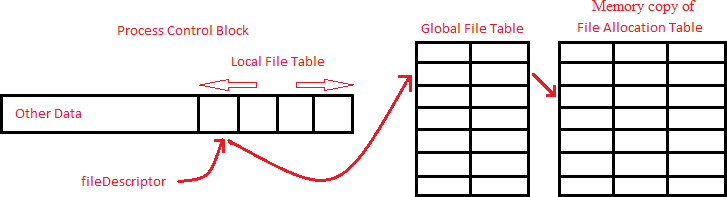
\includegraphics[scale=0.65]{pics/access_method}
	\caption{Diagram showing the method of accessing FAT entry}
	\label{access_scheme}
\end{figure}

\subsection{INT 4}
The file system call \textit{Write} invoke INT 4. INT 4 handles these system calls as follows.

\textbf{Write :} This system call is used to write data into an open file. \\
Syntax : \texttt{int Write(fileDescriptor, mem\_loc, numWords)} 
\footnote{It is advisable to have  a maximum of 1 block for any data file if it has to be modified using \texttt{write} system call since if the modification spans multiple blocks the entire procedure to access a block (outlined above) has to be repeated.} \\
Syscall no : \counter{syscall}
\index{File System Calls!Write}
\begin{itemize}
	\item First of all, the basic block of the file specified by the \texttt{fileDescriptor} is loaded into the scratchpad. This is done in the following way:
	\begin{itemize}
		\item The \texttt{fileDescriptor} is used first to access the local file table entry of the file. An appropriate error is returned if the \texttt{fileDescriptor} is out of the range specified.
		\item This local file table entry is then used to access the global file table entry of the file.
		\item Then the FAT index field in the global file table entry is used to access the FAT entry of the file.
		\item The basic block address present in the FAT entry is then used load the basic block (containing block list and file header info) into the scratchpad. Refer figure~\ref{access_scheme}.
	\end{itemize}	
	
	\item The lseek position present in the GFT entry and \texttt{numWords} are used to index the block list in the basic block to find the block numbers of the block(s) to be written into. \footnote{The data block to which the lseek position is pointing to is got by dividing lseek by the block size. \\
	The data block number calculated above is used to index the block list in the basic block to get the exact location of the data block in the disk. The data block is then loaded from the disk into the scratchpad. \\
	If the words to be read are split across multiple data blocks, the above procedure is repeated.}
	
	\item Each time the block to be written into is loaded into the scratchpad before performing the write operation.
	
	\item After loading the specified block, the content to be written is copied from the user memory location (\texttt{mem\_loc}) into this block. If \texttt{mem\_loc} is out of the address space of the process, an appropriate error code is returned.
	
	\item If the write operation exhausts all the currently allocated blocks, new blocks are allocated as required. This is done in the following way.
	\begin{itemize}
		\item The memory copy of the disk free list \index{Disk Free List!Memory copy} is used to get the block number of a free block.
		\item A new basic block entry is created using this free block number and added to the block list of the basic block. Successive write operations are then performed the usual way.
	\end{itemize}
	
	\item Once all the write operations are over for that block, it is stored back into the disk.
	
	\item The updated copies of FAT \index{File Allocation Table!Memory copy} and disk free list 
	\index{Disk Free List!Memory copy} in the memory are committed to the disk.
	
	\item The return value of this system call is the number of words successfully written. In case of an error, an appropriate error code is returned.
\end{itemize}


\section{Process System Calls}
\label{procsyscall}
\index{Process System Calls}
\textit{Process system calls} are used by a process when it has to duplicate itself, execute a new process in its place or when it has to terminate itself. There are three process system calls. An interrupt is associated with each system call. All the necessary arguments for a system call are available in the user stack with the system call number as the last argument.\\

\noindent Interrupt specifications for different \textit{Process system calls} are as follows:

\subsection{INT 5}
The process system call \textit{Fork} invokes INT 5. INT 5 handles these system calls as follows.

\textbf{Fork :}  This system call is used to create a new process having the same code area, data area and list of open files as that of the process which invoked this system call.

The new process that is created is known as the \emph{child} process, and the process which invoked this system call is known as its \emph{parent}.

The register values in the PCB of the child process are initialized with the current register contents.\\
Syntax : \texttt{int Fork()} \\
Syscall no : \counter{syscall}
\index{Process System Calls!Fork}
\begin{itemize}
	\item A vacant entry is searched for in the \emph{Ready list}.
	\item If no entry is found, in the case when there are already 12 processes that are active, an appropriate error code is returned.
	\item The index of this vacant ready list entry is the PID for the child process that is created.
	\item The PID entry in the PCB of the child process is updated with this new PID.
	\item All the registers (except PID) and the local file table of the parent process is replicated in the PCB of the child process.
	\item The code pages, the data page and the stack page of the parent process is replicated for this child process.
	\item The control is returned back to the parent process.
	\item The return value of this system call is the PID of the child process.
\end{itemize}

\subsection{INT 6}
The process system call \textit{Exec} invokes INT 6. INT 6 handles these system calls as follows.

\textbf{Exec :}  This system call is used to load the program, whose name is specified in the argument, in the memory space of the current process and start its execution .\\
Syntax : \texttt{int Exec(filename)} \\
Syscall no : \counter{syscall}
\index{Process System Calls!Exec}
\begin{itemize}
	\item The entire process area of the currently executing process is replaced by that of the program specified in the argument (\texttt{filename}). 
	\item If the file specified by \texttt{filename} is not an executable \footnote{Executables in {\ESIM} must end with an extension \texttt{.sim}} then, an appropriate error code is returned.
	\item The memory copy of the FAT \index{File Allocation Table!Memory copy} is searched to get the location of the basic block of the file specified by \texttt{filename}, which is then loaded into the scratchpad.
	\item This is then used to get the location in the disk of the blocks of the file to be loaded.
	\item The 2 code blocks and 1 data block of the file are loaded from the disk into the corresponding locations in the memory of the code blocks and data block of the current process.
	\item The PCB of the current process is modified to hold the values for that of the new process. The PID and page table, however, remains unchanged.\footnote{This is because the mappings remain the same as the code blocks and data block of the specified executable are loaded into the same locations as of the current process. Since, no new process table entry is created, the PID also remains the same.}
	\item The return value of this system call is 1 in case of a failure. Nothing is returned in case of a success.
\end{itemize}

\subsection{INT 7}
The process system call \textit{Exit} invokes INT 7. INT 7 handles this system call as follows.
\textbf{Exit :}  This system call is used to terminate the execution of the process which invoked it and removes it from the memory . It loads the next available process.\\
Syntax :  \texttt{Exit()}  \\
Syscall no : \counter{syscall}
\index{Process System Calls!Exit}
\begin{itemize}
	\item The entire address space of the currently executing process is set free by setting a value 0 in the memory free list corresponding to the pages occupied by that process.
	
	\item The local file table is traversed and the global file table entry is removed.
	
	\item The ready list entry corresponding to this process is set to zero thereby releasing all the data structures used by the process (fig~\ref{fig:ds with process}).
	
	\item The ready list is then searched for the next available process. The INIT process is excluded in this search.\footnote{This can be accomplished by setting the PID of INIT process as 0 and searching only the entries from 1--11 in the ready list.} If one such process is found, the PID is updated with the index of this entry in the ready list. If no such process is found, then the PID is set to the index of the INIT process in the ready list.
	
	\item All the registers of the machine are initialised with their corresponding values obtained from the PCB of the process specified by the new PID.
	
	\item The process switches from \textit{Kernel mode} to \textit{User mode}.
\end{itemize}

\section{INIT Process}
The INIT process is the first user process loaded by the OS on the OS startup. INIT was previously defined in chapter~\ref{chp:osstartup} as a normal user program. Since multiprogramming functionalities have been added to the OS, INIT must be modified. The modified specification of INIT process is as follows:
\begin{itemize}
	\item  It provides an interface for the users to run other user programs.
	\item The user enters the name of a valid executable file (which should be made available in the disk) in the shell. If the specified file is not found, an appropriate error code is returned.
	\item If the specified executable file is found, the INIT process forks and does exec on the that file.
	\item Entering the keyword HALT instead of the name of an executable file invokes the Shutdown system call.
\end{itemize}

All the user processes other than INIT are added to entries 1-11 of the ready queue keeping the 0th entry (corresponding to INIT) untouched. INIT loads the first process and thereafter all context switches occur among the other processes in the ready queue. INIT is switched back only when the ready queue (entries 1-11) is free so that the user can load another executable file via the shell. 

%\appendix TODO !!
%\section{Simple Integer Machine (SIM) architecture}
% \chapter{System Programmer's manual}
% The following diagram illustrates the interaction among various modules that have been written in the code. 
% 
%  \begin{figure}[htp!]
% 	  \centering
% % 	  \includegraphics[scale=0.55]{pics/spm}
% 	  \caption{Interaction among various modules in the implementation}
% 	  \label{fig:spm}
% 	  \end{figure}
% 
% Each module performs a specific function which has been well documented in the code. All variables and data structures that are used are suitably named and proper constants have been defined for anything that has a fixed value like location in memory of the various data structures and other machine constants. 



\end{document}